\documentclass[final,t]{beamer}
\mode<presentation>
{
  \usetheme{GINSFNASAposter}
}
\usepackage[orientation=landscape,size=custom,width=140,height=100,scale=1.2]{beamerposter}


% additional settings
\setbeamerfont{itemize}{size=\normalsize}
\setbeamerfont{itemize/enumerate body}{size=\normalsize}
\setbeamerfont{itemize/enumerate subbody}{size=\normalsize}

% additional packages
\usepackage{times}
\usepackage{subfigure}
\usepackage{verbatim} 
\usepackage{wasysym}
\usepackage{exscale}
\usepackage{multicol}
\usepackage{booktabs,array}
\usepackage{natbib}
\usepackage[english]{babel}
\usepackage[latin1]{inputenc}

\bibliographystyle{chicago}

\usepackage{iftex}
\ifXeTeX
\usepackage{fontspec}
\setmainfont[Ligatures=TeX]{Times New Roman}
\fi

\def\newblock{\hskip .11em plus .33em minus .07em} % for natbib and beamer IMPORTANT
\listfiles
\graphicspath{{figures/}}
% Display a grid to help align images
%\beamertemplategridbackground[1cm]




\title{\huge Contribution of the Greenland Ice Sheet to sea-level over the next millennium}
\author[Aschwanden et al.]{Andy Aschwanden\inst{1}, Mark A Fahnestock\inst{1}, Martin Truffer\inst{1}, Regine Hock\inst{1}, Ruth Mottram\inst{2}, S. Abbas Khan\inst{3 }, and Constantine Khroulev\inst{1}}
\institute[GI]{
\inst{1} Geophysical Institute, University of Alaska Fairbanks, USA\\
\inst{2} Danish Meteorological Institute, Copenhagen, Denmark\\
\inst{3} DTU Space, Copenhagen, Denmark
}
%\date[Aug. 31 , 2007]{Aug. 31 , 2007}

% abbreviations
\usepackage{xspace}
\makeatletter
\DeclareRobustCommand\onedot{\futurelet\@let@token\@onedot}
\def\@onedot{\ifx\@let@token.\else.\null\fi\xspace}
\def\eg{{e.g}\onedot} \def\Eg{{E.g}\onedot}
\def\ie{{i.e}\onedot} \def\Ie{{I.e}\onedot}
\def\cf{{c.f}\onedot} \def\Cf{{C.f}\onedot}
\def\etc{{etc}\onedot}
\def\vs{{vs}\onedot}
\def\wrt{w.r.t\onedot}
\def\dof{d.o.f\onedot}
\def\etal{{et al}\onedot}
\makeatother


%%%%%%%%%%%%%%%%%%%%%%%%%%%%%%%%%%%%%%%%%%%%%%%%%%%%%%%%%%%%%%%%%%%%%%%%%%%%%%%%%%%%%%%%%%%%%%%%%%%%%%%%%%%%

\begin{document}
\begin{frame}[fragile]{} 

  \vspace{2em}
  \centering \LARGE{How will Greenland look like a thousand years from now? Choose your future!}

  \begin{columns}[T]

    \begin{column}{.65\linewidth}
      \begin{figure}
        \centering
        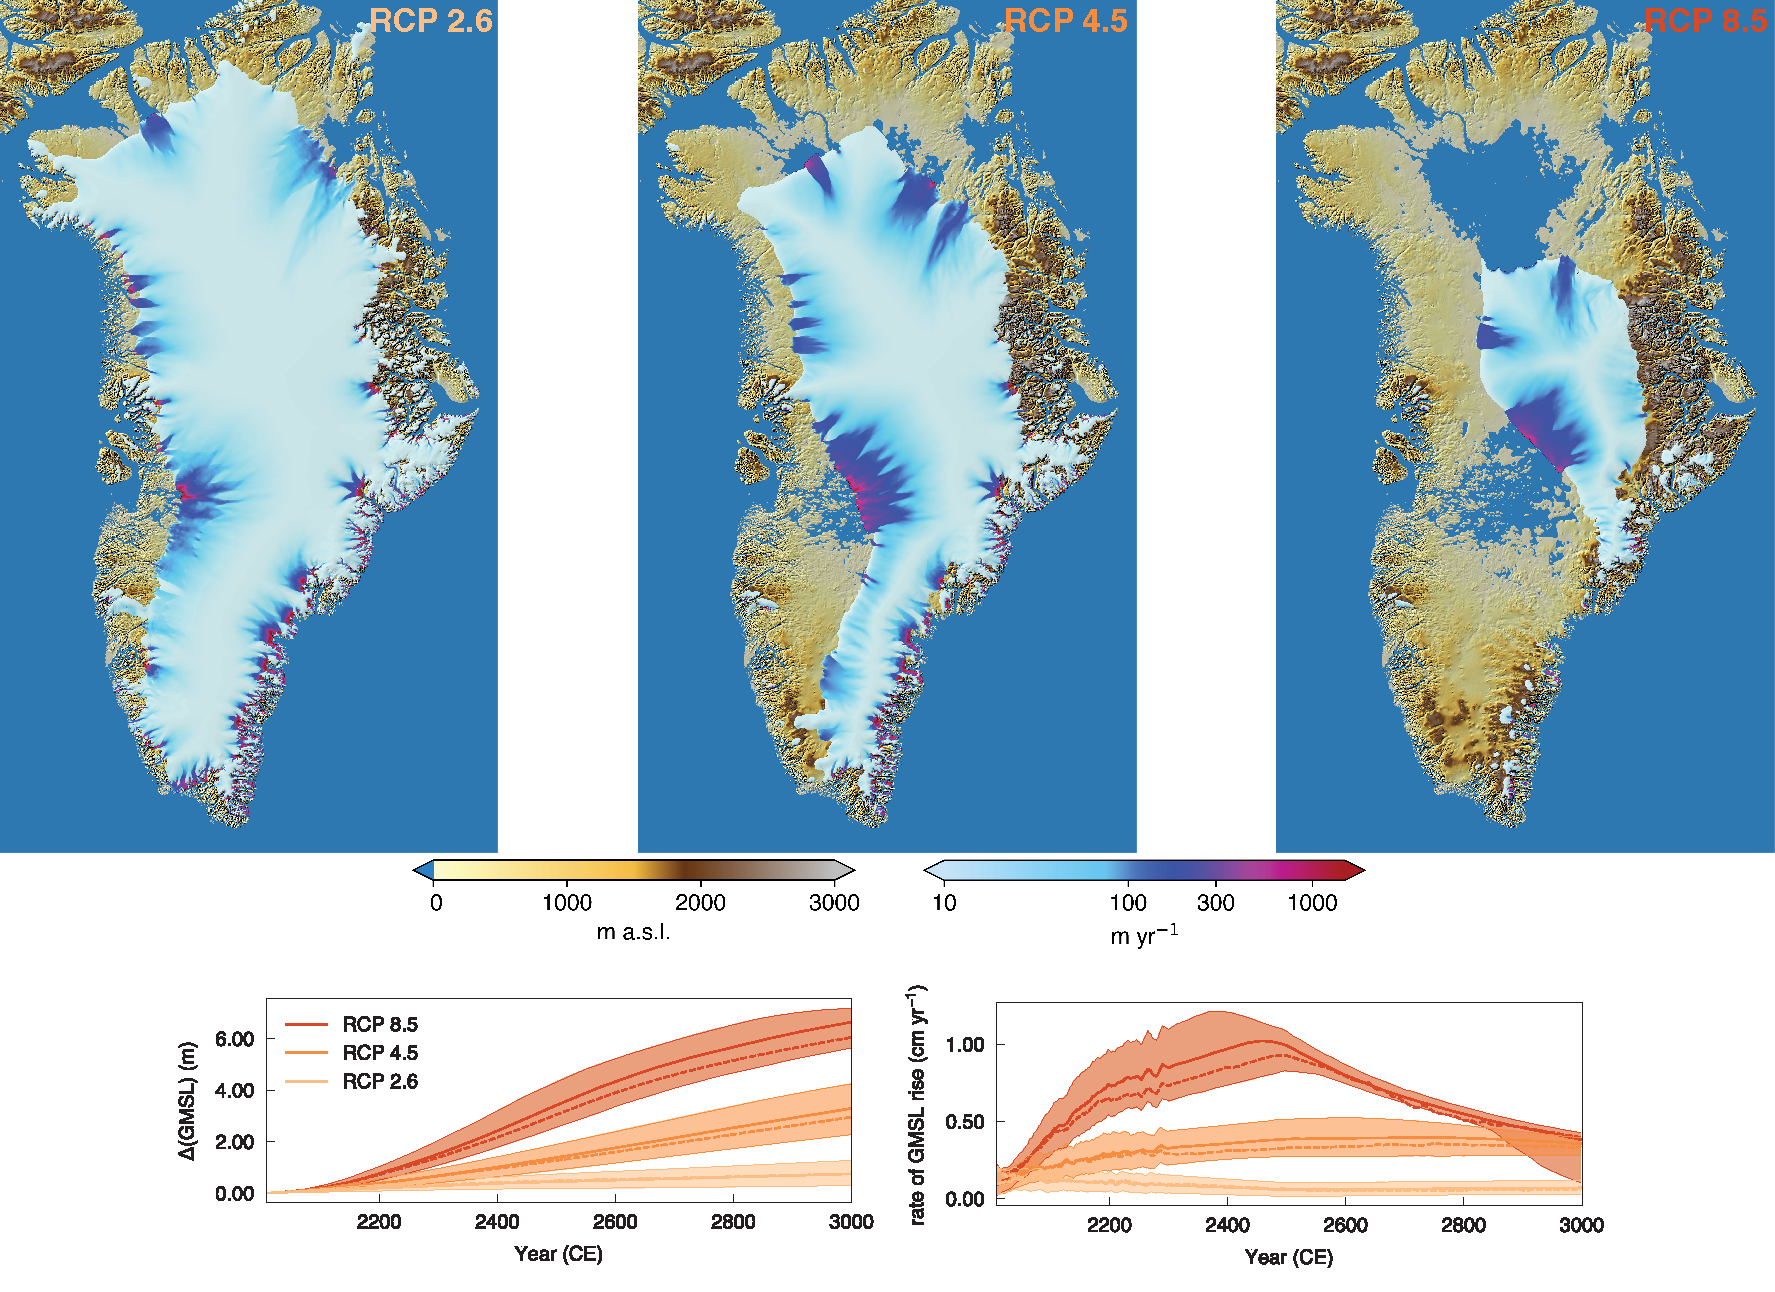
\includegraphics[width=\textwidth]{rcp-final-states-agu} 
        \caption{How Greenland could look like a thousand years from now under RCP Scenarios 2.6, 4.5, and 8.5. Upper panel: surface speeds. Lower left panel: Cumulative contribution to Global Mean Sea Level (GMSL). Lower right panel: Rates (11-yr running means) of GMSL rise. Solid line is 50-percentile (median) with uncertainties shaded between 16th percentile and 84th percentile of a 1,000 ensemble member simulations and the dashed line is an calibrated parameter simulation.}
        \label{fig:sg-results}
      \end{figure}
      
    \end{column}

\end{columns}

\end{frame}

\end{document}


%%%%%%%%%%%%%%%%%%%%%%%%%%%%%%%%%%%%%%%%%%%%%%%%%%%%%%%%%%%%%%%%%%%%%%%%%%%%%%%%%%%%%%%%%%%%%%%%%%%%
%%% Local Variables: 
%%% mode: latex
%%% TeX-PDF-mode: t
%%% End: 